\documentclass[a4paper,titlepage,12pt]{scrartcl}	%El modo de documento es para la numeración.

\usepackage{graphicx} %Imágenes
\usepackage[utf8]{inputenc} %Tildes
\usepackage[spanish,es-tabla]{babel} %Español, es-table: llamar tablas en vez de cuadros
\usepackage[breaklinks=true]{hyperref} %Hiperenlaces
\usepackage{amssymb, amsmath, amsbsy} %Símbolos matemáticos
\usepackage{float} %Mover las imágenes usando [H]
\usepackage{eurosym} %Símbolo de euro \euro
\usepackage{listings} %Código
\usepackage{listingsutf8} %Tildes en listings

\numberwithin{figure}{section} %Hace que la primera figura de cada sección X sea X.1
\numberwithin{table}{section} %Hace que la primera tabla de cada sección X sea X.1

\begin{document}
	\lstset{inputencoding=utf8/latin1} %Tildes en listlings
	\begin{titlepage}
		\begin{center}
			\begin{figure}[htb]
				\begin{center}
					
\includegraphics[width=12cm]{./Portada/ugr.png}
				\end{center}
			\end{figure}

			\vspace*{0.8cm}
			\begin{Large}
				\textbf{Grado en Ingeniería Informática.}\\
			\end{Large}
			\begin{Huge}
				\vspace{1.5cm}
				\textbf{Práctica 5.} \\
			\end{Huge}
			\vspace*{0.76cm}
			\rule{100mm}{0.1mm}\\
			\vspace*{0.5cm}
			\begin{large}
				\textbf{Nombre de la asignatura:}\\
				Ingeniería de Servidores.\\
				\vspace*{0.5cm}
				\textbf{Realizado por:}\\
				Néstor Rodríguez Vico \\

				\vspace*{2cm}
				\begin{figure}[htb]
					\begin{center}
						
\includegraphics[width=5cm]{./Portada/etsiit.png}
					\end{center}
				\end{figure}
				\vspace*{-0.6cm}
				ESCUELA TÉCNICA SUPERIOR DE INGENIERÍAS INFORMÁTICA Y DE TELECOMUNICACIÓN.\\
				\rule{20mm}{0.1mm}\\
				\vspace*{0.6cm}
				Granada, \today.
			\end{large}
		\end{center}
	\end{titlepage}
	
	%--------------Indices--------------
	\tableofcontents
	\clearpage
	\listoffigures %Imagenes
%	\listoftables %Tablas
	\clearpage
	%----------------------------------
	
	%%%%%%%%%%%%%%%%%%%%%%%%%%%%%%%%%%%%%%%%%%%%%%%%%%%%
	%%%%%%%%%%%%%%%%%%%% Cuestión 1 %%%%%%%%%%%%%%%%%%%%
	%%%%%%%%%%%%%%%%%%%%%%%%%%%%%%%%%%%%%%%%%%%%%%%%%%%%	
	\section[Cuestión 1: Al modificar los valores del kernel de este modo, no logramos que persistan después de reiniciar la máquina. ¿Qué archivo hay que editar para que los cambios sean permanentes?]{Cuestión 1: Al modificar los valores del kernel de este modo, no logramos que persistan después de reiniciar la máquina. ¿Qué archivo hay que editar para que los cambios sean permanentes?}
	
	Como podemos ver en la página de RedHat \cite{kernel} debemos editar el fichero \textit{/etc/sysctl.config}. Hay que tener cuidado al modificar archivos de configuración, así que lo más inteligente sería copiar dicho archivo antes de modificarlo, para ello ejecutamos \textit{sudo cp /etc/sysctl.conf /etc/sysctl.conf.original}. De esta manera, en caso de que haya algún problema, sólo tendríamos que restaurar la copia de seguridad. Una vez modificado el archivo, hacemos los cambios permanentes. En mi caso he cambiado el domino del kernel. Este proceso lo podemos ver en la figura \ref{1-1}.
	
	\begin{figure}[H]
		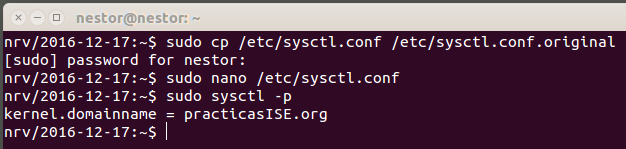
\includegraphics[width=\linewidth]{./Imagenes/1-1.png}
		\vspace{-0.5cm}
		\caption[Cambio de un parámetro del kernel.]{Cambio de un parámetro del kernel.}
		\label{1-1}
	\end{figure}
	
	%%%%%%%%%%%%%%%%%%%%%%%%%%%%%%%%%%%%%%%%%%%%%%%%%%%%
	%%%%%%%%%%%%%%%%%%%% Cuestión 2 %%%%%%%%%%%%%%%%%%%%
	%%%%%%%%%%%%%%%%%%%%%%%%%%%%%%%%%%%%%%%%%%%%%%%%%%%%	
	\section[Cuestión 2: Cuestión 2 : ¿Con qué opción se muestran todos los parámetros modificables en tiempo de ejecución? Elija dos parámetros y explique, en dos líneas, qué función tienen.]{Cuestión 2: ¿Con qué opción se muestran todos los parámetros modificables en tiempo de ejecución? Elija dos parámetros y explique, en dos líneas, qué función tienen.}
	
	Como podemos ver en la página del manual de \textit{sysctl} \cite{sysctl_man} esto se consigue ejecutando \textit{sysctl -a}. Parte de dichos parámetros lo podemos ver en la figura \ref{2-1}.
	
	\begin{figure}[H]
		\centering
		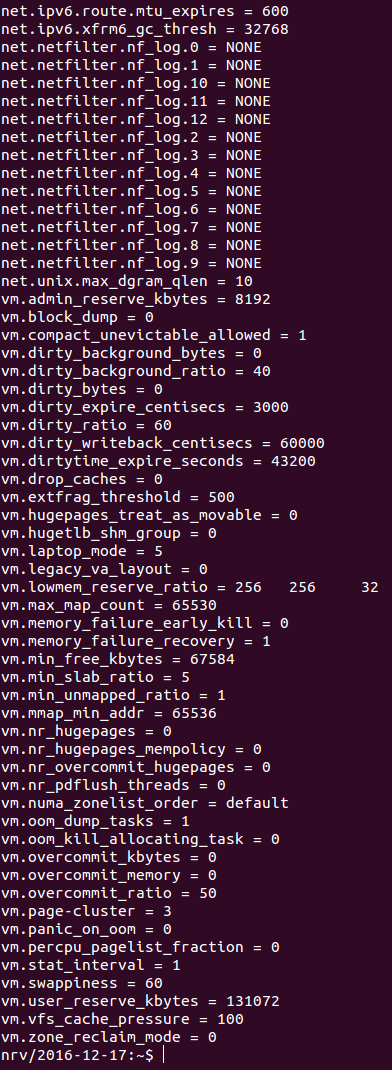
\includegraphics[scale=0.4]{./Imagenes/2-1.png}
		\caption[Parte de los parámetros modificables en tiempo de ejecución.]{Parte de los parámetros modificables en tiempo de ejecución.}
		\label{2-1}
	\end{figure}
	
	Para entender que hacen los parámetros del kernel podemos visitar la documentación oficial del kernel \cite{kernel_doc}. Los parámetros que yo he elegido son \textit{net.core.netdev\_budget} y \textit{vm.max\_map\_count}. El valor de dichos parámetros lo podemos ver en la figura \ref{2-2}:
	
	\begin{figure}[H]
		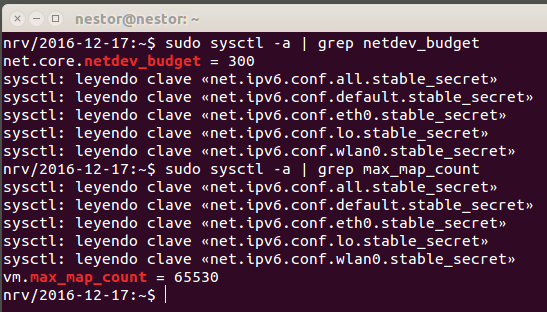
\includegraphics[width=\linewidth]{./Imagenes/2-2.png}
		\vspace{-0.5cm}
		\caption[Valores de \textit{net.core.netdev\_budget} y \textit{vm.max\_map\_count}.]{Valores de \textit{net.core.netdev\_budget} y \textit{vm.max\_map\_count}.}
		\label{2-2}
	\end{figure}
	
	La función del parámetro \textit{net.core.netdev\_budget} la podemos ver en la página oficial del kernel, en la sección destinada a la parte de red \cite{net}. Dicho parámetro indica el número máximo de paquetes que pueden ser aceptados en un ciclo de sondeo. \\
	
	La función del parámetro \textit{vm.max\_map\_count} la podemos ver en la página oficial del kernel, en la sección destinada a la parte de la memoria virtual \cite{vm}. Dicho parámetro indica el número máximo de áreas de memoria que un proceso puede tener.
	
	%%%%%%%%%%%%%%%%%%%%%%%%%%%%%%%%%%%%%%%%%%%%%%%%%%%%
	%%%%%%%%%%%%%%%%%%%% Cuestión 3 %%%%%%%%%%%%%%%%%%%%
	%%%%%%%%%%%%%%%%%%%%%%%%%%%%%%%%%%%%%%%%%%%%%%%%%%%%
	\section[Cuestión 3: ]{Cuestión 3: }
	\subsection[a) Realice una copia de seguridad del registro y restáurela, ilustre el proceso con capturas.]{a) Realice una copia de seguridad del registro y restáurela, ilustre el proceso con capturas.}
	
	El proceso de copia y restauración del registro lo podemos ver en la página oficial de Windows \cite{registro_windows}. Los pasos que he seguido son los siguientes:
	\begin{enumerate}
		\item Pulsamos en inicio, le damos a buscar y escribimos \textit{regedit}, como podemos ver en la figura \ref{3a-1}.
		\item Pulsamos sobre \textit{Archivo}, luego elegimos \textit{Exportar}. Nos aparecerá la ventana que podemos ver en la figura \ref{3a-2}. Ahora elegimos la ubicación y el nombre de la copia y le damos a \textit{Guardar}.
		\item Para restaurar el registro, le damos a \textit{Archivo}, luego elegimos \textit{Importar}. Nos aparecerá la ventana que podemos ver en la figura \ref{3-3a}. Ahora elegimos la ubicación de la copia y le damos a \textit{Abrir}.
		\item Esta operación puede que nos de el error que vemos en la figura \ref{3a-4} y sólo se restaurará parte del registro. En caso de querer que se restaure todo, podemos pulsar la tecla \textit{F8} al encender la máquina y nos aparecerá un menú como el que podemos ver en la figura \ref{3a-5}. En dicho menú elegimos la opción \textit{La última configuración válida conocida (avanzada)} y se restaurará el registro que había la última vez que se encendió la máquina correctamente.
	\end{enumerate}
	
	\begin{figure}[H]
		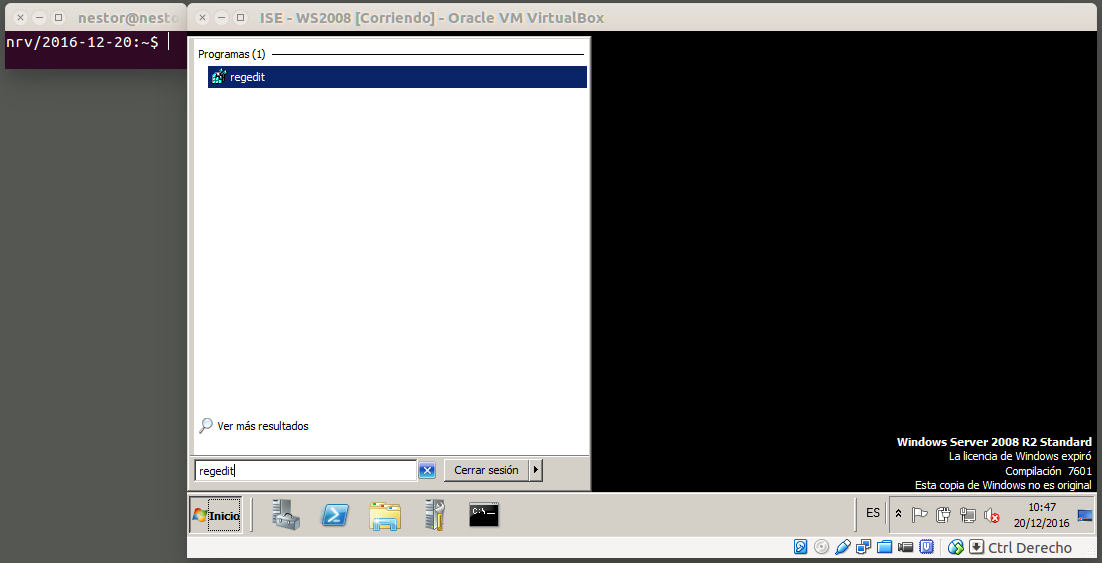
\includegraphics[width=\linewidth]{./Imagenes/3a-1.png}
		\vspace{-0.5cm}
		\caption[Abrimos el editor del registro.]{Abrimos el editor del registro.}
		\label{3a-1}
	\end{figure}
	
	\begin{figure}[H]
		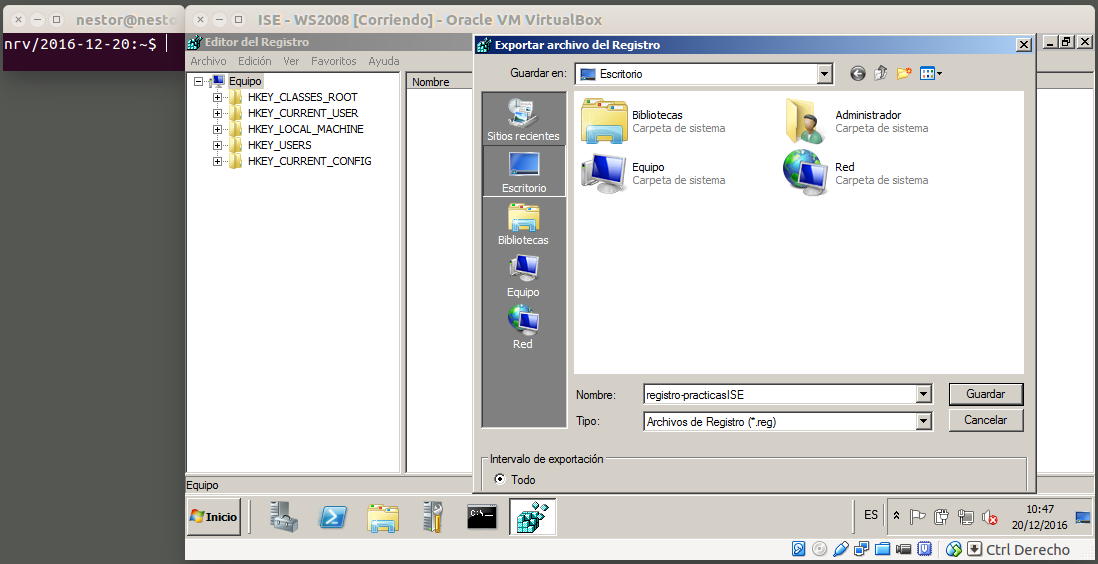
\includegraphics[width=\linewidth]{./Imagenes/3a-2.png}
		\vspace{-0.5cm}
		\caption[Exportamos el registro.]{Exportamos el registro.}
		\label{3a-2}
	\end{figure}
	
	\begin{figure}[H]
		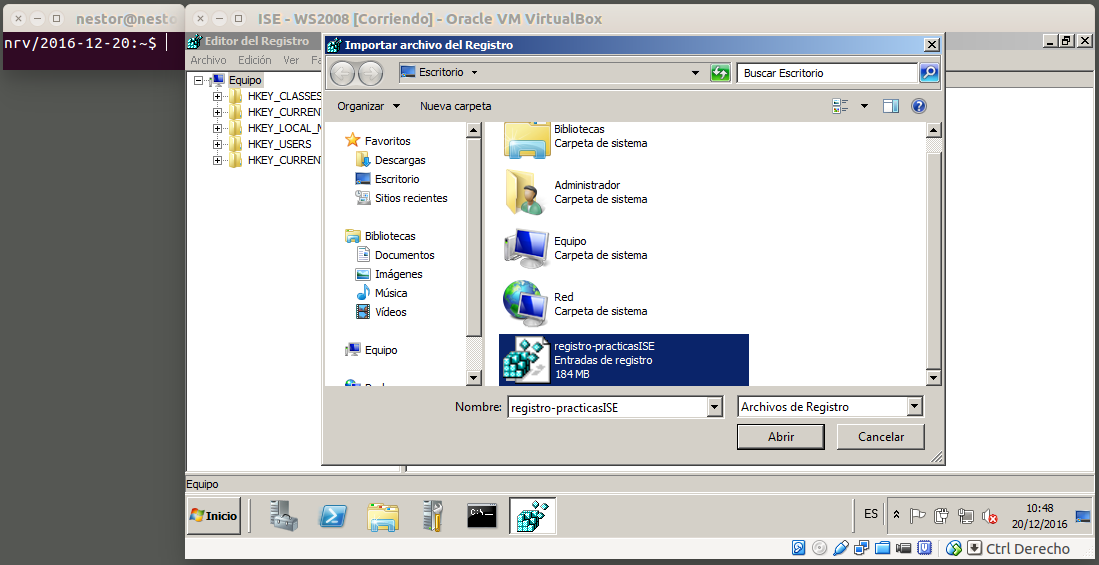
\includegraphics[width=\linewidth]{./Imagenes/3a-3.png}
		\vspace{-0.5cm}
		\caption[Importamos el registro.]{Importamos el registro.}
		\label{3a-3}
	\end{figure}
	
	\begin{figure}[H]
		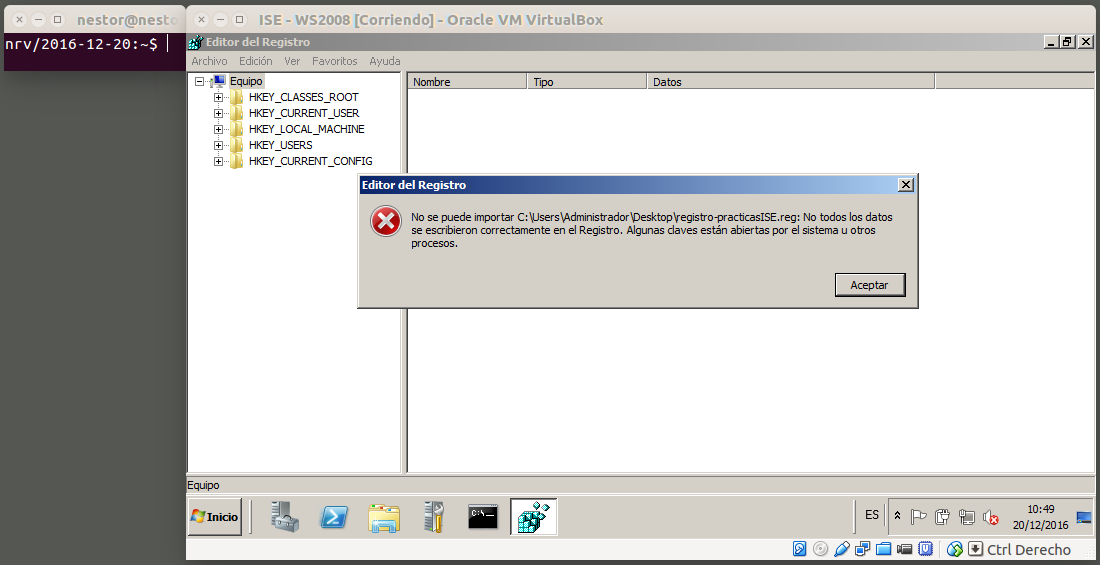
\includegraphics[width=\linewidth]{./Imagenes/3a-4.png}
		\vspace{-0.5cm}
		\caption[Error en la importación del registro.]{Error en la importación del registro.}
		\label{3a-4}
	\end{figure}
	
	\begin{figure}[H]
		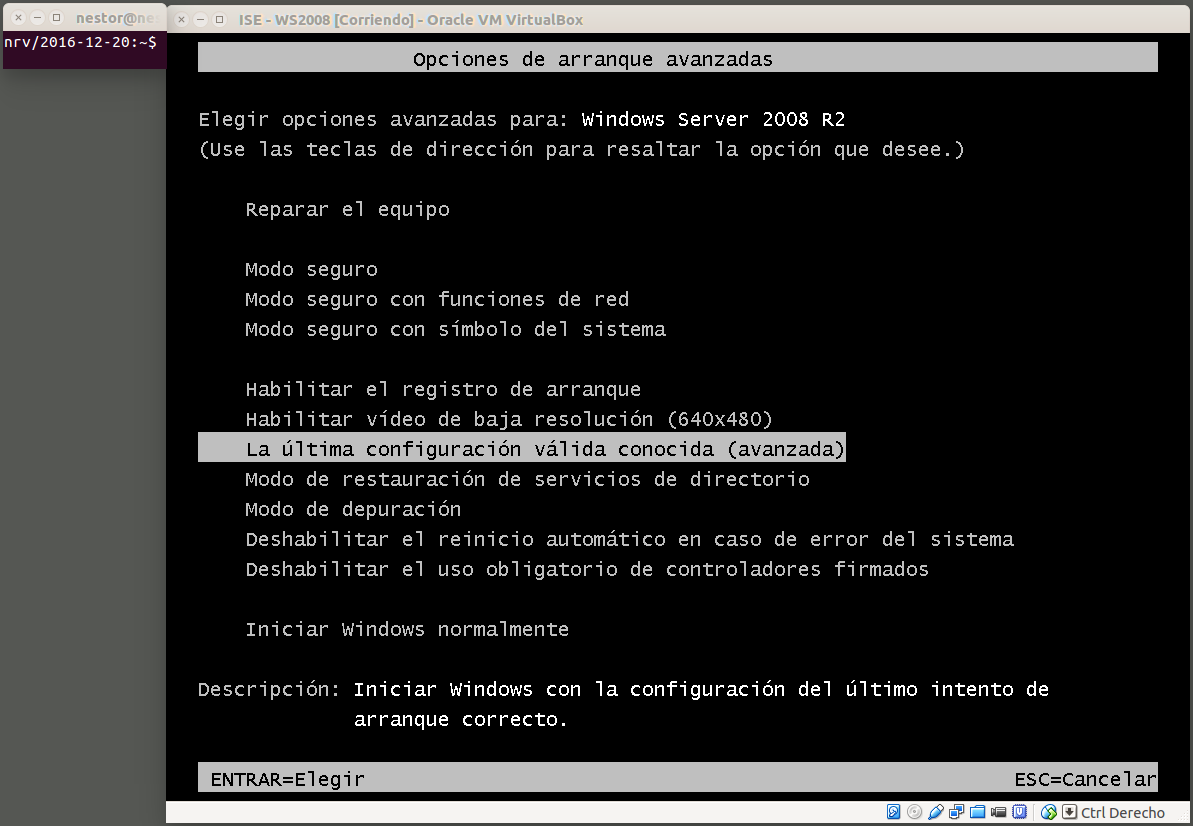
\includegraphics[width=\linewidth]{./Imagenes/3a-5.png}
		\vspace{-0.5cm}
		\caption[Opciones de arranque avanzadas.]{Opciones de arranque avanzadas.}
		\label{3a-5}
	\end{figure}
	
	\subsection[b) Abra una ventana mostrando el editor del registro.]{b) Abra una ventana mostrando el editor del registro.}
	
	Para abrir el editor del registro pulsamos en inicio, le damos a buscar y escribimos \textit{regedit}, como podemos ver en la figura \ref{3b-1}. A continuación le damos a la tecla \textit{Intro} y se abrirá el editor del registro, como podemos ver en la figura \ref{3b-2}.
	
	\begin{figure}[H]
		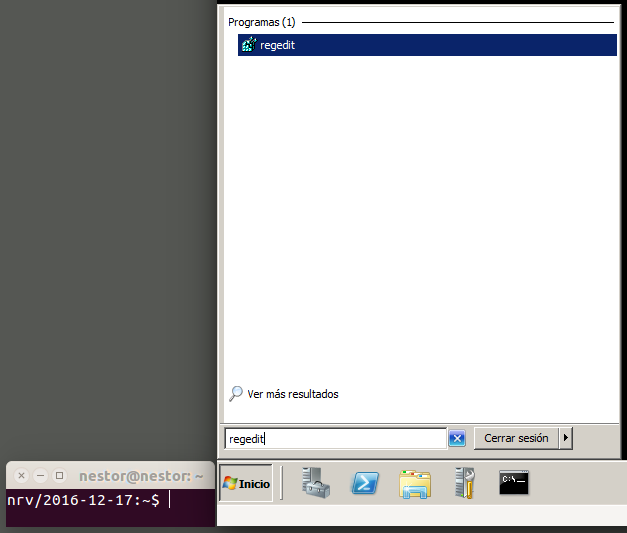
\includegraphics[width=\linewidth]{./Imagenes/3b-1.png}
		\vspace{-0.5cm}
		\caption[Como abrir el editor del registro.]{Como abrir el editor del registro.}
		\label{3b-1}
	\end{figure}

	\begin{figure}[H]
		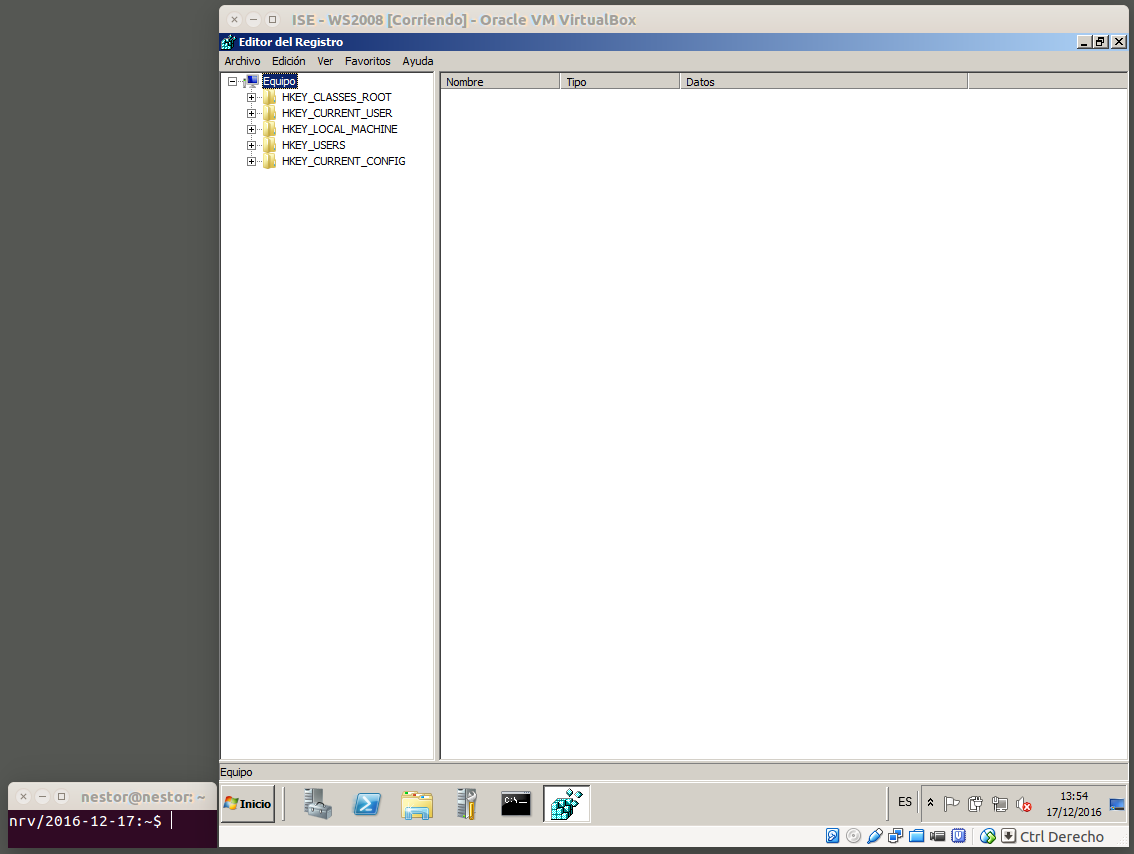
\includegraphics[width=\linewidth]{./Imagenes/3b-2.png}
		\vspace{-0.5cm}
		\caption[Editor del registro.]{Editor del registro.}
		\label{3b-2}
	\end{figure}
	
	%%%%%%%%%%%%%%%%%%%%%%%%%%%%%%%%%%%%%%%%%%%%%%%%%%%%
	%%%%%%%%%%%%%%%%%%%% Cuestión 4 %%%%%%%%%%%%%%%%%%%%
	%%%%%%%%%%%%%%%%%%%%%%%%%%%%%%%%%%%%%%%%%%%%%%%%%%%%
	\section[Cuestión 4: Enumere qué elementos se pueden configurar en Apache y en IIS para que Moodle funcione mejor.]{Cuestión 4: Enumere qué elementos se pueden configurar en Apache y en IIS para que Moodle funcione mejor.}
	
	Para ver que elementos podemos modificar para mejorar el rendimiento nos dirigimos a la página de Moodle \cite{moodle}. En el caso de \textit{Apache} dichas recomendaciones son:
	\begin{itemize}
		\item En caso de estar usando \textit{Apache} en Windows Server es recomendable instalar \textit{Apache Lounge} \cite{apachelounge} en vez de \textit{Apache}, ya que se han reportado mejoras de rendimiento con esta versión no oficial de \textit{Apache}.
		\item Cambiar el valor de \textit{MaxClients}. El nuevo valor sería: \textit{MaxClients = Memoria total disponible * 80\% / Memoria máxima para el proceso apache}. La memoria máxima para el proceso apache suele ser 10MB, pero \textit{Moodle} puede usar hasta 100MB. En caso de querer poner un valor superior a 256 sería necesario cambiar también el valor de \textit{ServerLimit}.
		\item Reducir el número de módulos que \textit{Apache} carga modificando el fichero \textit{httpd.conf} o el fichero \textit{apache2.conf}, según el sistema operativo usado.
		\item Usar la última versión de \textit{Apache}.
		\item En caso de usar un sistema operativo basado en Unix/Linux, reducir el valor de \textit{MaxRequestsPerChild} a un valor entre 20 y 30.
		\item Para servidores con alta carga cambiar el valor de \textit{KeepAlive} a \textit{Off} o reducir el valor de \textit{KeepAliveTimeout} a un valor entre 2 y 5.
		\item Una alternativa a cambiar el valor de \textit{KeepAlive} es configurar un \textit{Reverse Proxy server} que almacene en la caché del servidor los archivos HTML y las imágenes.
		\item Si no se usa un fichero de acceso \textit{.htaccess}, cambiar el valor de la variable \textit{AllowOverride} a \textit{None}.
		\item Establecer el valor de \textit{DirectoryIndex} correctamente para evitar la negación de contenido.
		\item Si no se está haciendo ninguna prueba sobre el servidor, cambiar el valor de \textit{ExtendedStatus} a \textit{Off} y desactivar \textit{mod\_info} y \textit{mod\_status}.
		\item Dejar \textit{HostnameLookups} a su valor por defecto (\textit{Off}).
		\item Cambiar el valor de \textit{TimeOut} a un valor entre 30 y 60 (segundos).
		\item En la directiva \textit{Options} evitar \textit{Options Multiviews}. Para reducir las entradas/salidas en disco hay que usar \textit{Indexes FollowSymLinks}.
	\end{itemize}
	
	En el caso de estar usando IIS las recomendaciones se realizan modificando la localización \textit{HKLM\textbackslash SYSTEM\textbackslash CurrentControlSet\textbackslash Services\textbackslash Inetinfo\textbackslash Parameters\textbackslash} en el registro. Las recomendaciones son:
	\begin{itemize}
		\item El equivalente a \textit{KeepAliveTimeout} es \textit{ListenBackLog} así que lo cambiamos a un valor entre 2 y 5.
		\item Cambiar el valor de \textit{MemCacheSize} para ajustarlo a la cantidad de memoria en Mb que ISS utilizará para su fichero de cache.
		\item Cambiar el valor de \textit{MaxCachedFileSize} para ajustarlo al tamaño máximo que tendrá un fichero en cache en bytes.
		\item Crear una nueva \textit{DWORD} llamado \textit{ObjectCacheTTL} para cambiar el tiempo (en milisegundos) que los objetos en caché serán mantenidos en memoria. El valor por defecto es 30000 milisegundos.		
	\end{itemize}
	
	%%%%%%%%%%%%%%%%%%%%%%%%%%%%%%%%%%%%%%%%%%%%%%%%%%%%
	%%%%%%%%%%%%%%%%%%%% Cuestión 5 %%%%%%%%%%%%%%%%%%%%
	%%%%%%%%%%%%%%%%%%%%%%%%%%%%%%%%%%%%%%%%%%%%%%%%%%%%
	\section[Cuestión 5: Ajuste la compresión en el servidor y analice su comportamiento usando varios valores para el tamaño de archivo a partir del cual comprimir. Para comprobar que está comprimiendo puede usar el navegador o comandos como curl (see url) o lynx. Muestre capturas de pantalla de todo el proceso.]{Cuestión 5: Ajuste la compresión en el servidor y analice su comportamiento usando varios valores para el tamaño de archivo a partir del cual comprimir. Para comprobar que está comprimiendo puede usar el navegador o comandos como curl (see url) o lynx. Muestre capturas de pantalla de todo el proceso.}
	
	Para ver como habilitar y configurar la compresión he seguido las indicaciones que podemos encontrar en la documentación oficial de Microsoft \cite{compresionISS}. Los pasos que he seguido son lo siguientes:
	\begin{enumerate}
		\item Para habilitar la compresión desde la interfaz gráfica abrimos el administrador de \textit{Internet Information Service}, para ello pulsamos en \textit{Inicio}, le damos a buscar y escribimos \textit{IIS} y abrimos el primer resultado, como podemos ver en la figura \ref{5-1}.
		\item Elegimos nuestro servidor, \textit{NESTOR} en mi caso, y buscamos \textit{Compresión}, tal y como podemos ver en la figura \ref{5-2}.
		\item Pinchamos sobre \textit{Habilitar compresión de contenido estático}. Para forzar al servidor a que comprima todos los archivos cambiamos el tamaño mínimo para comprimir un archivo a 1. Este proceso lo podemos ver en la figura \ref{5-3}.
		\item Una vez hemos configurado la compresión, la probamos con \textit{curl}. Para ver como usarlo he mirado la documentación oficial \cite{curl} y las páginas del manual \cite{curl2}. Para ejecutarlo usamos el comando \textit{curl -I -H `Accept-Encoding: gzip,deflate' direccionIP} desde mi máquina remota. En mi caso, como podemos ver en la figura \ref{5-4} la dirección IP de mi servidor es \textit{192.168.56.101} (máquinas conectadas en modo \textit{host-only}) así que ejecutamos \textit{curl -I -H `Accept-Encoding: gzip,deflate' 192.168.56.101}, como podemos ver en la figura \ref{5-4}. El argumento \textit{-I} sirve para indicar que sólo se capten las cabeceras HTTP. El argumento \textit{-H} seguido de \textit{`Accept-Encoding: gzip,deflate'} sirve para indicar una cabecera extra cuando se está obteniendo una página web. Además, indicamos que use \textit{gzip} y forzamos al servidor a comprimir los datos con \textit{deflate}. En la figura \ref{5-4} podemos ver que el tamaño del contenido es 457  bytes y podemos ver que en el atributo \textit{Content-Encodeing} tiene el valor \textit{gzip}, tal y como indicamos en el comando.
		\item A continuación desactivamos la compresión y ejecutamos el mismo comando, como podemos ver en la figura \ref{5-5}. En la figura \ref{5-5} también podemos ver que ahora el tamaño del contenido es de 689 bytes.
	\end{enumerate}
		
	\begin{figure}[H]
		\centering
		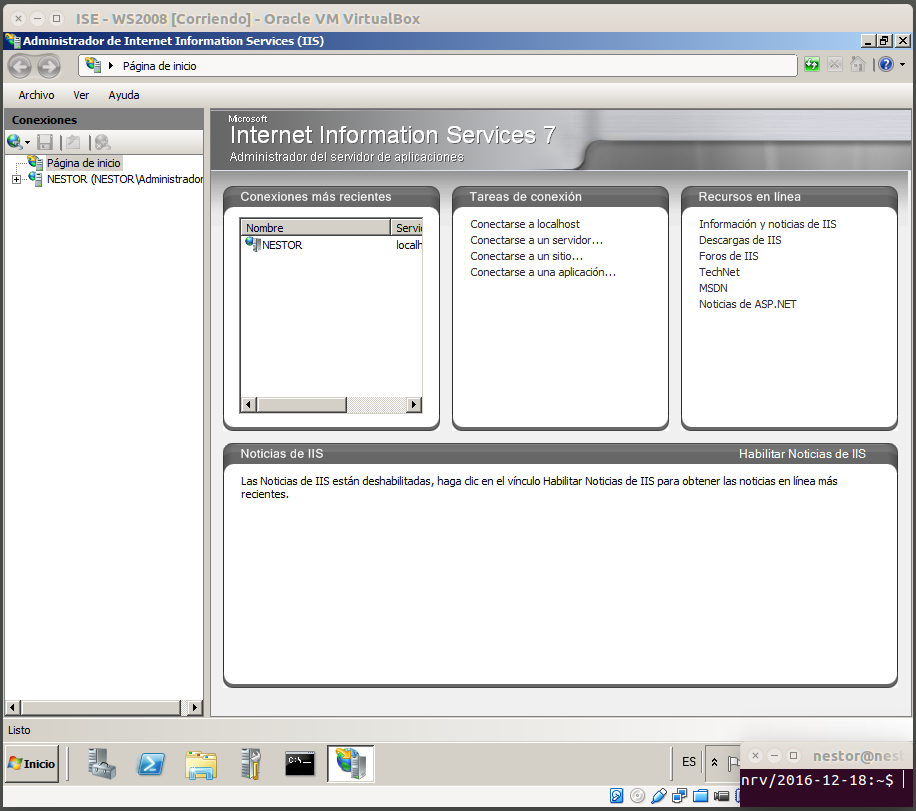
\includegraphics[scale=0.33]{./Imagenes/5-1.png}
		\caption[Administrador de \textit{Internet Information Service}.]{Administrador de \textit{Internet Information Service}.}
		\label{5-1}
	\end{figure}
		
	\begin{figure}[H]
		\centering
		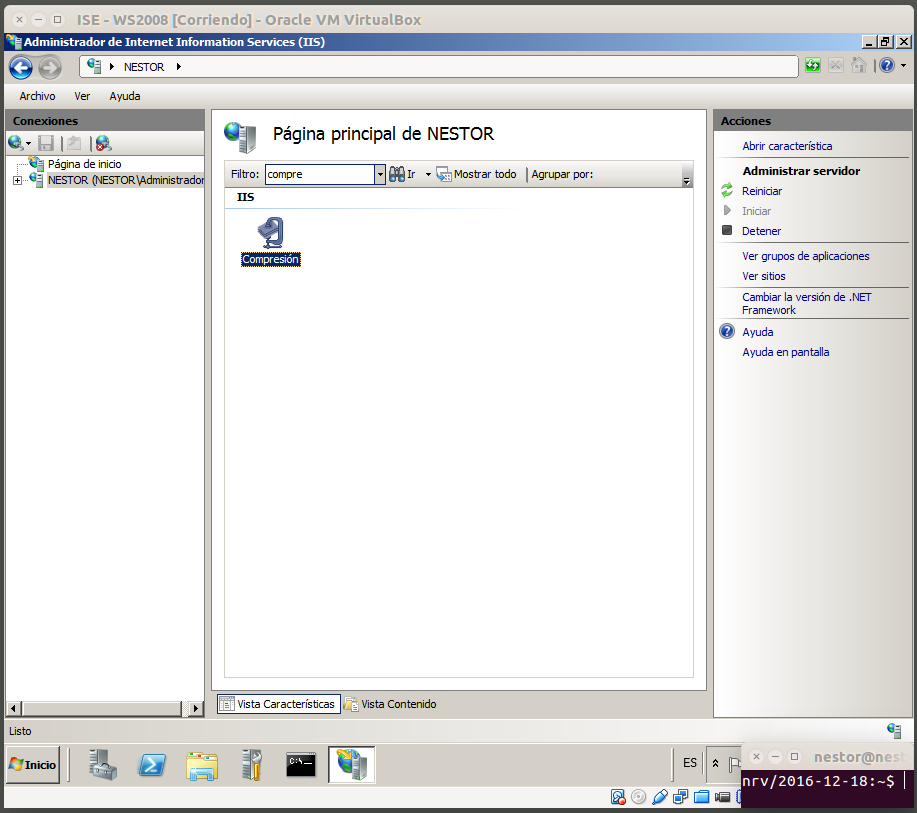
\includegraphics[scale=0.33]{./Imagenes/5-2.png}
		\caption[Sección de compresión.]{Sección de compresión.}
		\label{5-2}
	\end{figure}
	
	\begin{figure}[H]
		\centering
		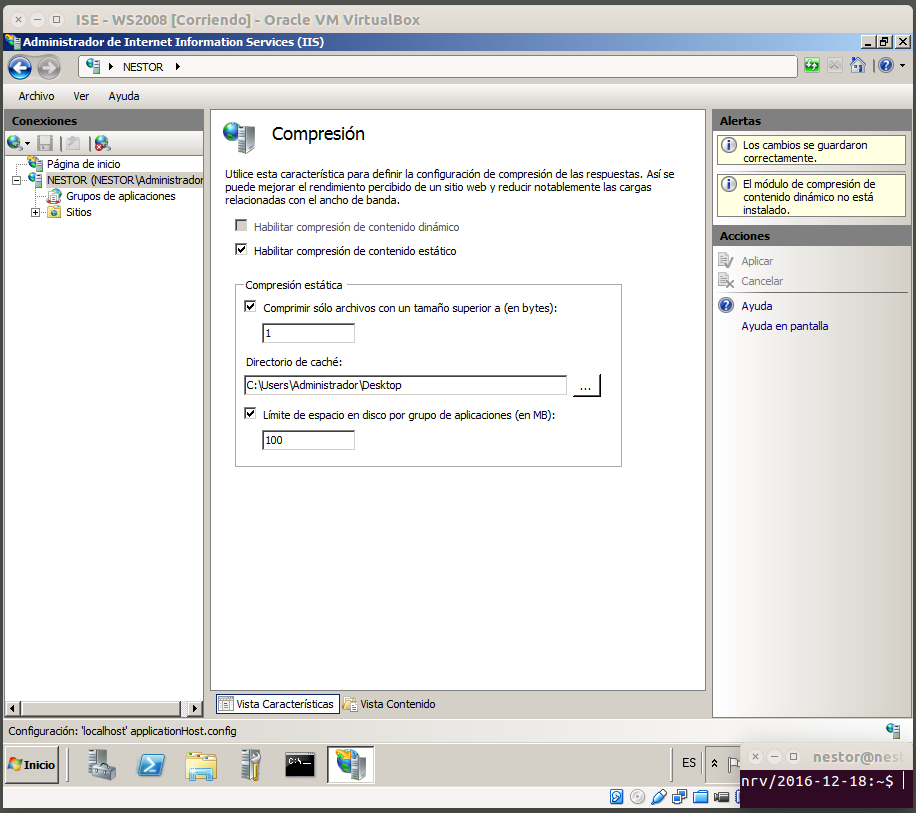
\includegraphics[scale=0.33]{./Imagenes/5-3.png}
		\caption[Configuración de la compresión.]{Configuración de la compresión.}
		\label{5-3}
	\end{figure}
	
	\begin{figure}[H]
		\centering
		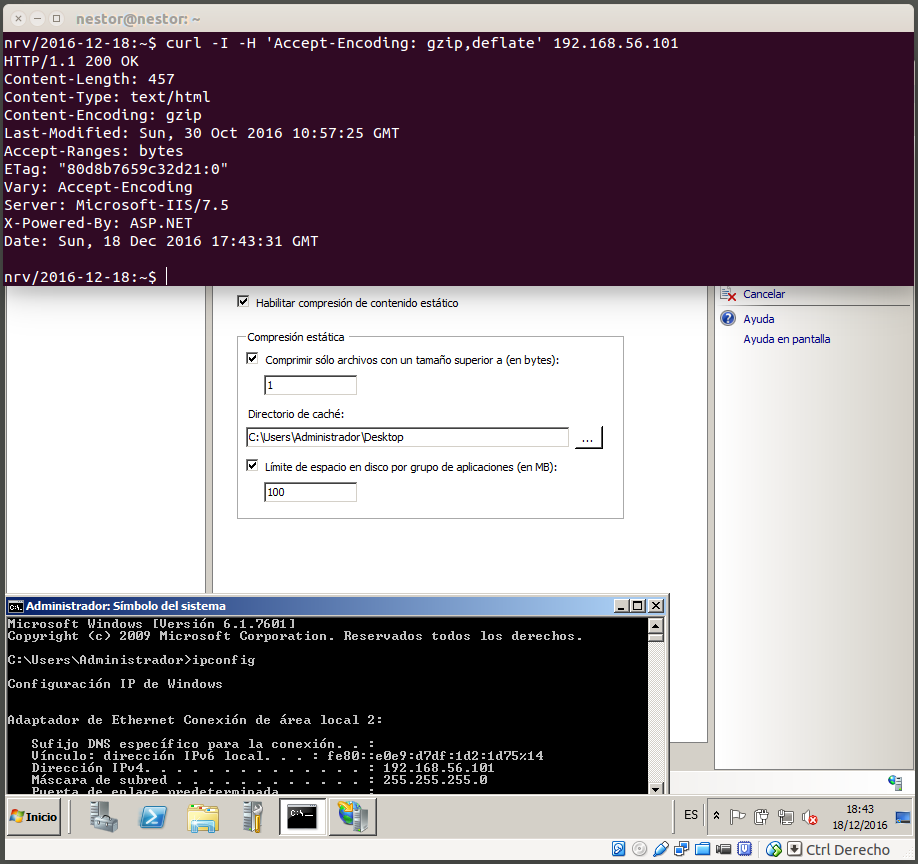
\includegraphics[scale=0.33]{./Imagenes/5-4.png}
		\caption[\textit{curl} con compresión activada.]{\textit{curl} con compresión activada.}
		\label{5-4}
	\end{figure}
	
	\begin{figure}[H]
		\centering
		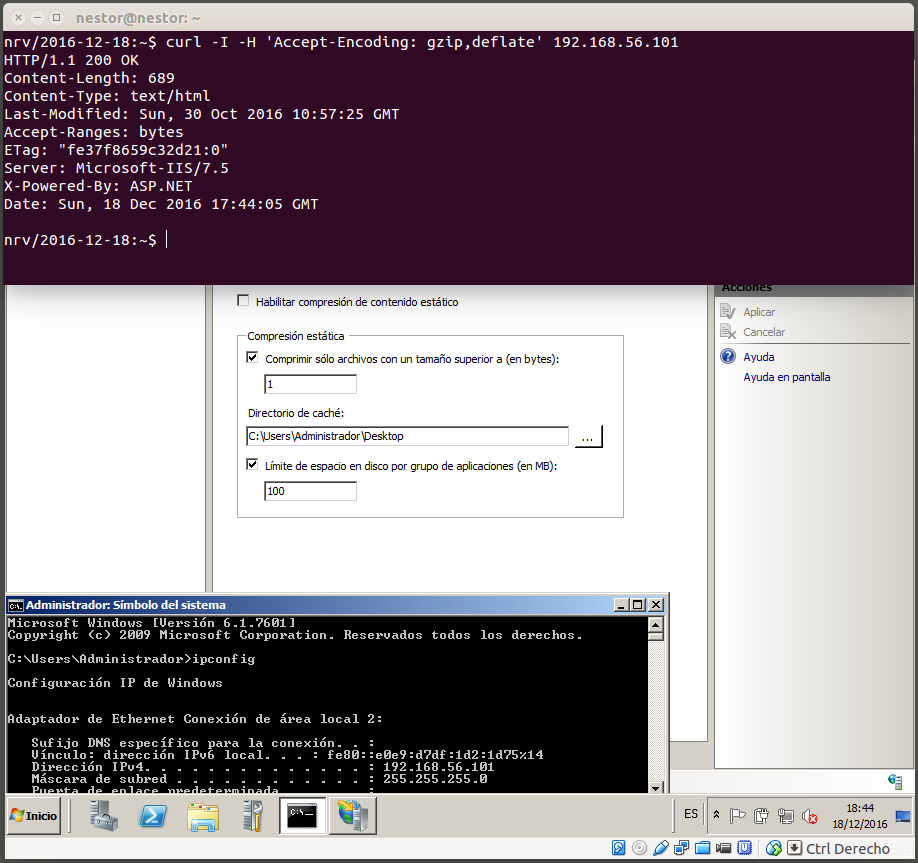
\includegraphics[scale=0.33]{./Imagenes/5-5.png}
		\caption[\textit{curl} con compresión desactivada.]{\textit{curl} con compresión desactivada.}
		\label{5-5}
	\end{figure}
	
	\section[Cuestión 6: Usted parte de un SO con ciertos parámetros definidos en la instalación (Práctica 1), ya sabe instalar servicios (Práctica 2) y cómo monitorizarlos (Práctica 3) cuando los somete a cargas (Práctica 4). Al igual que ha visto cómo se puede mejorar un servidor web (Práctica 5 Sección 3.1), elija un servicio (el que usted quiera) y modifique un parámetro para mejorar su comportamiento. \textbf{6.b)} Monitorice el servicio antes y después de la modificación del parámetro aplicando cargas al sistema (antes y después) mostrando los resultados de la monitorización.]{Cuestión 6: Usted parte de un SO con ciertos parámetros definidos en la instalación (Práctica 1), ya sabe instalar servicios (Práctica 2) y cómo monitorizarlos (Práctica 3) cuando los somete a cargas (Práctica 4). Al igual que ha visto cómo se puede mejorar un servidor web (Práctica 5 Sección 3.1), elija un servicio (el que usted quiera) y modifique un parámetro para mejorar su comportamiento. \textbf{6.b)} Monitorice el servicio antes y después de la modificación del parámetro aplicando cargas al sistema (antes y después) mostrando los resultados de la monitorización.}
	
	Lo que voy a realizar es comparar dos sistemas de archivos con idea de ver cuál sería más recomendable para usar en nuestro servidor. Para ello voy a realizar escrituras y lecturas en un disco duro y medir el tiempo empleado. Si esto lo hiciésemos sobre un disco duro virtual de \textit{VirualBox} los datos podrían no ser realmente fiables así que lo voy a hacer sobre un dispositivo de almacenamiento externo, un \textit{pendrive} de 2GB. \footnote{El programa en C++ que he realizado para realizar los test se encuentra dentro de la carpeta \textit{Archivos auxiliares} bajo el nombre \textit{``filesystem.cpp''}.} El código empleado es el siguiente: \\
	
	\begin{lstlisting}[frame=single, basicstyle=\footnotesize, label={filesystem.cpp}, breaklines=true]
#include <iostream>
#include <omp.h>
#include <iostream>
#include <fstream>
#include <stdio.h>
#include <string.h>

using namespace std;

int main(int argc, char *argv[]){
	double t_lectura1, t_escritura1, t_lectura2, t_escritura2, t_lectura, t_escritura;
	int i, hebra = -1;
	string line1, line2, line3, line4;
	char file1[100];
	char file2[100];
	char file3[100];
	char file4[100];

	strcpy(file1, argv[1]);	strcat(file1, ``file1.txt'');
	strcpy(file2, argv[1]);	strcat(file2, ``file2.txt'');
	strcpy(file3, argv[1]);	strcat(file3, ``file3.txt'');
	strcpy(file4, argv[1]);	strcat(file4, ``file4.txt'');

	cout << file1 << endl;
	cout << file2 << endl;
	cout << file3 << endl;
	cout << file4 << endl;

	omp_set_num_threads(4);

	ofstream output_file1(file1);
	ofstream output_file2(file2);
	ofstream output_file3(file3);
	ofstream output_file4(file4);

	#pragma omp parallel private(i)
	{
	//Medida de tiempo
	#pragma omp single
	{
		t_escritura1 = omp_get_wtime();
	}
	#pragma omp for
	for(i=0;i<25000000; i++){
		hebra = omp_get_thread_num();
		switch(hebra)
		{
		case 0:
		output_file1 << ``Iteracion " << i << `` ABCDEFGHIJKLMNOPQRSTUVWXYZ_0123456789 * Hebra 0 \n'';
		break;
		case 1:
		output_file2 << ``Iteracion " << i << `` ABCDEFGHIJKLMNOPQRSTUVWXYZ_0123456789 * Hebra 1 \n'';
		break;
		case 2:
		output_file3 << ``Iteracion " << i << `` ABCDEFGHIJKLMNOPQRSTUVWXYZ_0123456789 * Hebra 2 \n'';
		break;
		case 3:
		output_file4 << ``Iteracion " << i << `` ABCDEFGHIJKLMNOPQRSTUVWXYZ_0123456789 * Hebra 3 \n'';
		break;
		}
	}
	//Medida de tiempo
	#pragma omp single
	{
		t_escritura2 = omp_get_wtime();
	}
	}

	output_file1.close();
	output_file2.close();
	output_file3.close();
	output_file4.close();

	ifstream input_file1(file1);
	ifstream input_file2(file2);
	ifstream input_file3(file3);
	ifstream input_file4(file4);

	#pragma omp parallel private(i)
	{
	//Medida de tiempo
	#pragma omp single
	{
		t_lectura1 = omp_get_wtime();
	}
	hebra = omp_get_thread_num();
	switch(hebra)
	{
	case 0:
	while(getline(input_file1, line1))
		line1.size();
	break;
	case 1:
	while(getline(input_file2, line2))
		line2.size();
	break;
	case 2:
	while(getline(input_file3, line3))
		line3.size();
	break;
	case 3:
	while(getline(input_file4, line4))
		line4.size();
	break;
	}
	//Medida de tiempo
	#pragma omp single
	{
		t_lectura2 = omp_get_wtime();
	}
	}

	input_file1.close();
	input_file2.close();
	input_file3.close();
	input_file4.close();

	t_escritura = t_escritura2 - t_escritura1;
	t_lectura = t_lectura2 - t_lectura1;

	cout << ``Tiempo de escritura en segundos: '' << t_escritura << endl;
	cout << ``Tiempo de lectura en segundos: '' << t_lectura << endl;

	return 0;
}
	\end{lstlisting}
	
	Para compilar el programa ejecutamos \textit{g++ filesystem.cpp -o filesystem -fopenmp} y lo ejecutamos con el comando \textit{sudo ./filesystem $<$ruta$>$}. El procedimiento va a ser el siguiente:
	\begin{enumerate}
		\item Formateamos el \textit{pendrive} usando el sistema de archivos \textit{ext3}, tal y como podemos ver en la figura \ref{6-ext3}.
		\item Ejecutamos el código en C++ pasándole como argumento la ruta de nuestro \textit{pendrive} y guardamos los tiempos, tal y como podemos ver en la figura \ref{6-ext3}.
		\item Formateamos el \textit{pendrive} usando el sistema de archivos \textit{ntfs}, tal y como podemos ver en la figura \ref{6-ntfs}.
		\item Ejecutamos el código en C++ pasándole como argumento la ruta de nuestro \textit{pendrive} y guardamos los tiempos, tal y como podemos ver en la figura \ref{6-ntfs}.
		\item Comparamos los tiempos para ver que sistema de archivos nos da mejor rendimiento.
	\end{enumerate}
	
	Para formatear el \textit{pendrive} ejecutamos \textit{sudo fdisk -l}, como podemos ver en la figura \ref{6-ext3}, para ver donde cual es la ruta de nuestro \textit{pendrive}. En mi caso está en \textit{dev/sdb/}. Lo formateamos con el sistema de archivos \textit{ext3} con el comando \textit{sudo mkfs.ext3 -F /dev/sdb}, como podemos ver en la figura \ref{6-ext3}. Para la segunda parte de la prueba desmontamos el \textit{pendrive} con el comando \textit{umount /dev/sdb} y lo formateamos con el sistema de archivos \textit{NTFS} ejecutando el comando \textit{sudo mkfs.ntfs -F /dev/sdb}. \\
	
	Como podemos ver en la figura \ref{6-ext3} el sistema de archivos \textit{ext3} nos da un tiempo de escritura de 2.39499 segundos y un tiempo de lectura de 0.594771 segundos, mientras que el sistema de archivos \textit{NTFS} nos da un tiempo de escritura de 7.13254 segundos y un tiempo de lectura de 1.1876 segundos. En el caso de tener que usar uno de los dos sistemas de archivos en nuestro servidor, si creemos que el uso del disco va a ser similar al que hemos reproducido en nuestro código, sería preferible usar \textit{ext3} sobre \textit{NTFS} ya que nos proporciona mejores tiempos para la misma tarea.
	
	\begin{figure}[H]
		\centering
		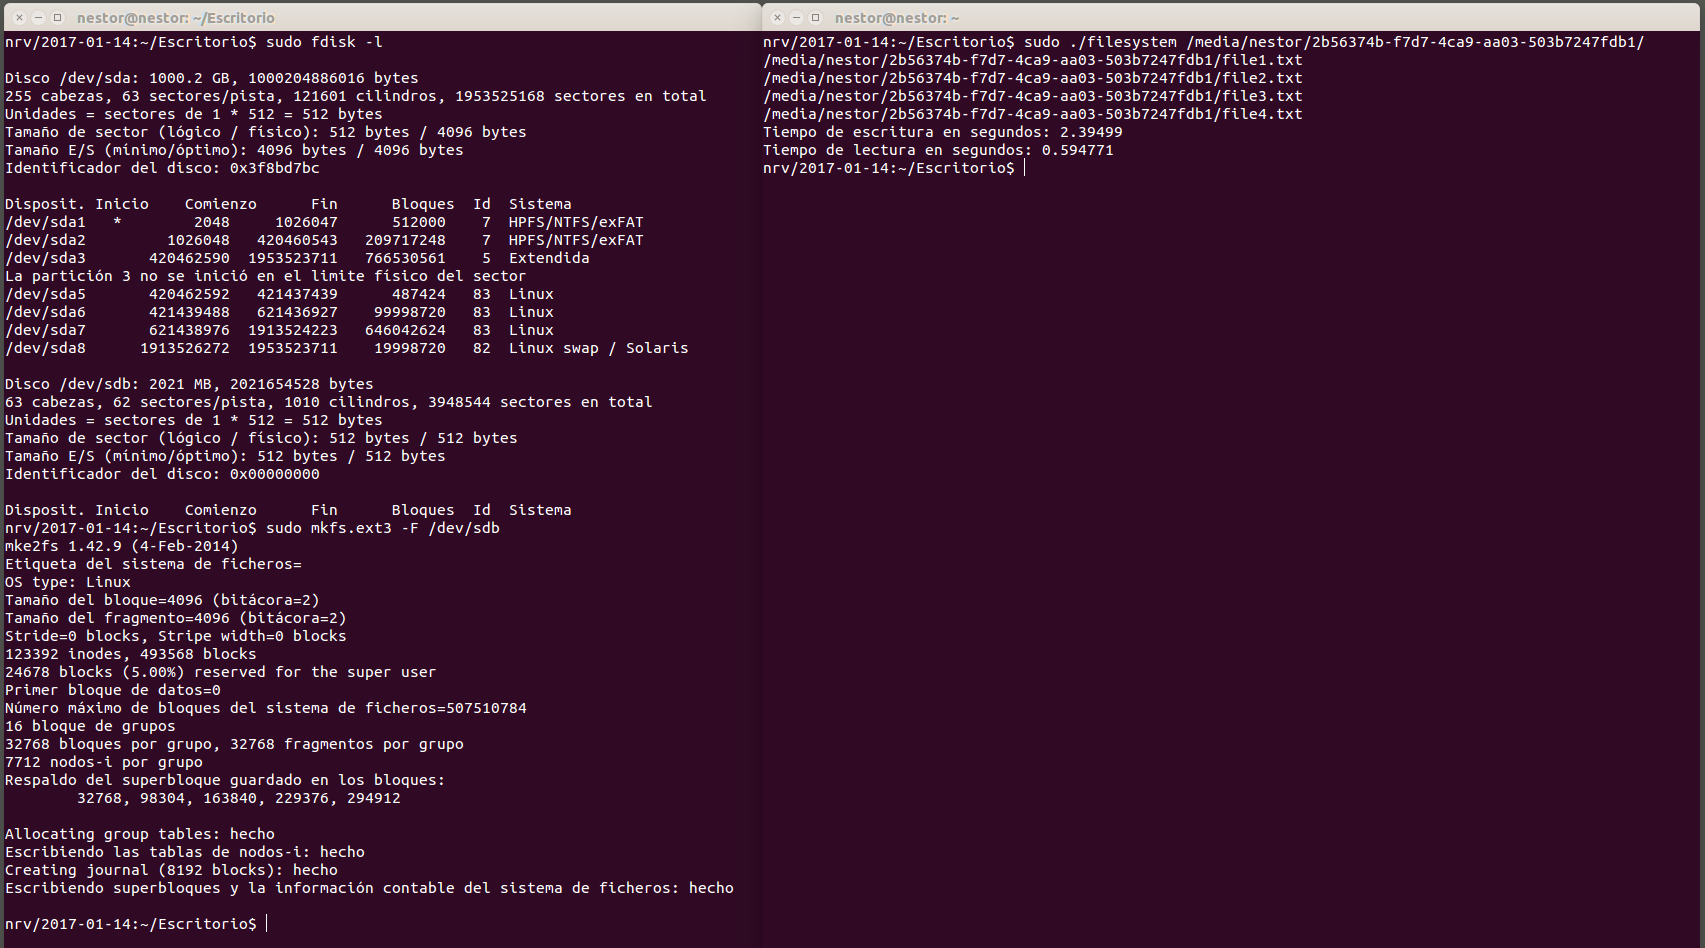
\includegraphics[width=\linewidth]{./Imagenes/6-ext3.png}
		\caption[\textit{ext3} como sistema de archivos y ejecución del programa.]{\textit{ext3} como sistema de archivos y ejecución del programa.}
		\label{6-ext3}
	\end{figure}
	
	\begin{figure}[H]
		\centering
		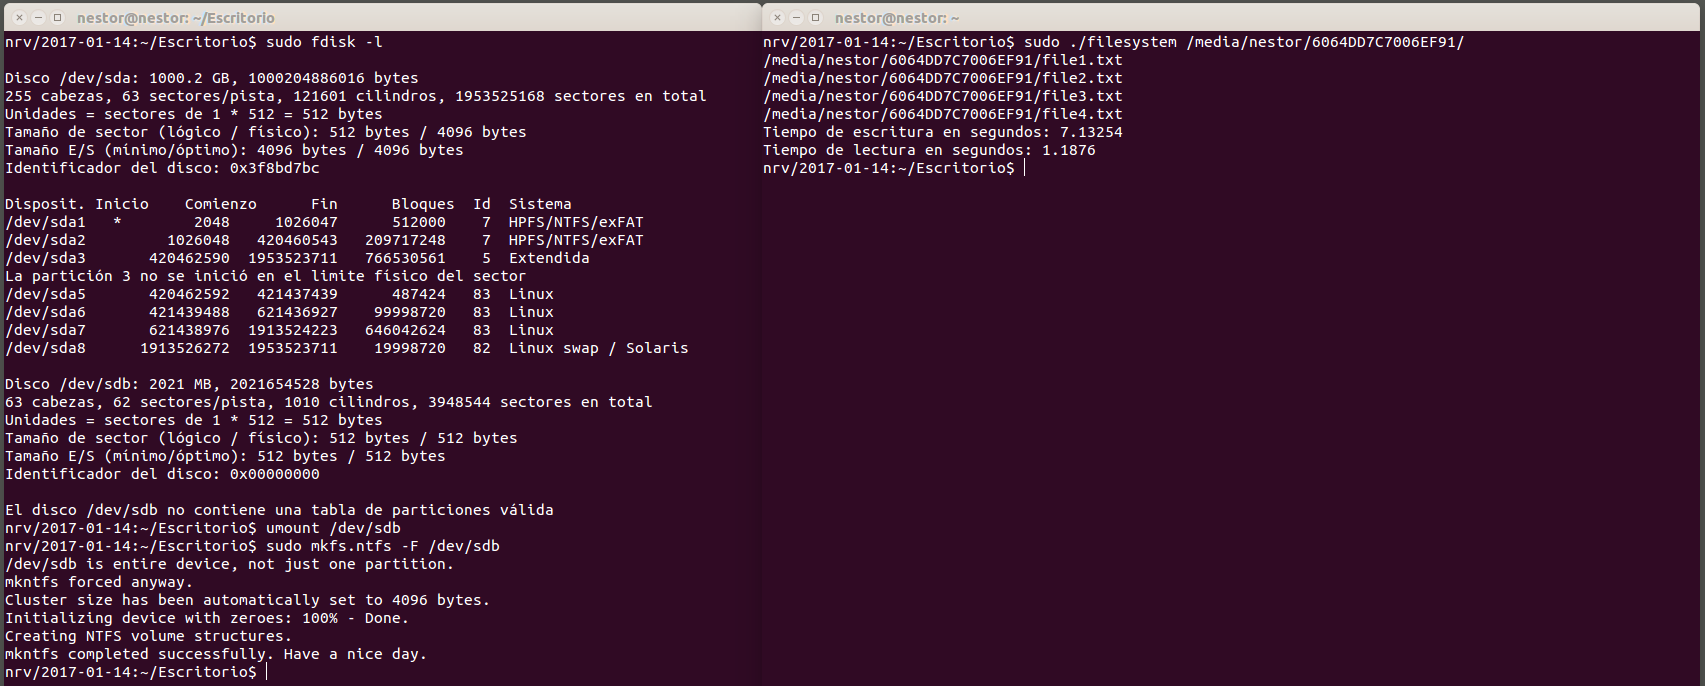
\includegraphics[width=\linewidth]{./Imagenes/6-ntfs.png}
		\caption[\textit{NTFS} como sistema de archivos y ejecución del programa.]{\textit{NTFS} como sistema de archivos y ejecución del programa.}
		\label{6-ntfs}
	\end{figure}
		
	\clearpage
	\bibliography{bibliografia}
	\bibliographystyle{ieeetr}
\end{document}